\documentclass{article}
\usepackage{blindtext}
\usepackage[utf8]{inputenc}
\usepackage{graphicx}
\usepackage{hyperref}
\usepackage[dvipsnames]{xcolor}
\graphicspath{ {/home/abhinav/Desktop/} }
 \hypersetup{
    colorlinks=true,
    linkcolor=blue,
    pdfpagemode=FullScreen,
}
\title{Documentation- \textbf{Newton-Raphson Method}}
\author{Abhinav Gupta}
\date{\today}

\begin{document}
 \tableofcontents
\maketitle
 
\section{Theory}
\subsection{Short Summary}
 
The Newton-Raphson Method is an iterative process for solving the root of the equation \(f(x)=0\).According to the method, starting with an initial guess of \(x_0\) ,apply the iterative formula

\[x_{n+1}=x_n-f(x_n)/f'(x_n)\]
where \(f\) denotes the derivative of the function. The iteration stops until you arrive at an acceptable limit \(|x_{n+1}- x_n|<\epsilon\), where \(\epsilon\) is some pre-specified tolerance value.

\[\includegraphics[scale=.5]{NewtonRaphson}\]
 
\subsection{Convergence of Newton-Raphson Method}
 
The tangent line approximation is—\textit{an approximation}. Let’s try to get
a handle on the error. Imagine a particle travelling in a straight line, and
let \(f(x)\) be its position at time \(x\). Then \(f'(x)\) is the velocity at time \(x\). If the acceleration of the particle were always 0, then the change in position from time \(x_0\) to time \(x_0+h\) would be \(hf'(x_0)\). So the position at time \(x_0+h\) would be \(f(x_0)+hf'(x_0)\)—-note that this is the tangent line approximation, which we can also think of as the zero-acceleration approximation.
\vspace{5mm}

 If the velocity varies in the time from \(x_0\) to \(x_0 + h\), that is, if the acceleration is not 0, then in general the tangent line approximation will not
correctly predict the displacement at time \(x_0 + h\). And the bigger the acceleration, the bigger the error. It can be shown that if \(f\) is twice differentiable then the error in the tangent line approximation is \((1/2)h^2f''(c)\) for some c between \(x_0\) and \(x_0 + h\). In particular, if \(|f''(x)|\) is large between \(x_0\) and \(x_0 + h\), then the error in the tangent line approximation is large. Thus we can expect large second derivatives to be bad for the Newton Method.
\vspace{5mm}

 These informal considerations can be turned into positive theorems about
the behaviour of the error in the Newton Method. For example, if \(|f''(x)/f'(x)|\) is not too large near \(r\), and we start with an \(x_0\) close enough to \(r\), the Newton Method converges very fast to \(r\). (Naturally, the theorem gives “not too
large,” “close enough,” and “very fast” precise meanings.)
The study of the behaviour of the Newton Method is part of a large and
important area of mathematics called Numerical Analysis.

\subsection{Where Newton’s method fails}

\begin{itemize}
    \item \textbf{\textit{Initial guess is a critical point of f(x) :}} the
definition of the Newton iteration function is
\[N(x) = x-f(x)/f'(x)\]
From this definition we see that \(N(x)\)will not exist if \(f'(x) = 0\). If we chose an
initial point where \(f'(x) = 0\), then Newton’s method will fail to converge to a root.
Similarly if \(f'(x_n) = 0\) for some iteration \(x_n\), then Newton’s method will also fail to converge to a root.

\item \textbf{\textit{No root to find :}} Another way in which Newton’s method will fail to converge
to the root of a function is if there is no root.
    
    \item \textbf{\textit{Periodic Cycle :}} A third way in which Newton’s method will fail to converge is if the initial guess or an iteration coincides with a cycle (i.e. a set of points occur repeatedly while approximating ).
\end{itemize}
\vspace{20mm}
\section{Why my answer is reasonable ??}
\[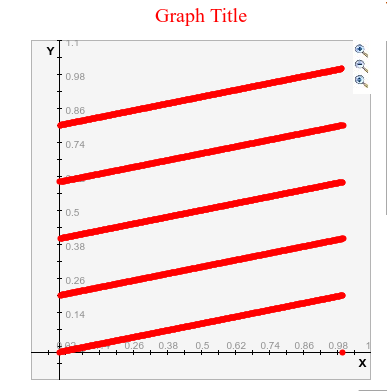
\includegraphics[scale=.4]{graph}\]
\begin{itemize}

    \item While choosing the initial point to start the approximation, I considered the graph of the function and chose such a integer point that was close to the root. As a result I considered a pair of consecutive integers for reference between whom the  root was graphically existing \textbf{(function had opposite signs on those integer points)}.Then I found the point among them on which the function derivative was large \textbf{(this was done to rectify slow movement of the approximations towards root)}.As there were 3 roots i choose three pair of such integer points for initialisation.Finally to stop the process at a certain point, tolerance was used and by the help of Newton-raphson method we reached to a approximate root of the equation.  
\end{itemize}
\section{Code and Output}
\[\includegraphics[scale=.3]{code}\]
\[\includegraphics[scale=.4]{output}\]
 
\end{document}